\createTaskHeader[Bridge Over Troubled Water][10]
Tommy si vo voľných chvíľach na záchode stavia mosty z~toaletných papierov.
Predstavme si, že máme postupne 2 až 10 rovnakých roliek toaleťáku (pre jednoduchosť si ich budeme predstavovať ako kvádriky).

Mostom budeme nazývať ľubovoľný útvar, ktorý je súvislý,
stabilný (nezrúti sa pod svojou vlastnou váhou) a dokáže preklenúť nenulovú vzdialenosť.
Kvôli jednoduchosti budeme uvažovať iba dvojrozmerný prípad (teda osi toaleťákov sú všetky zvislé a v~jednej rovine).
Oba konce mostov sú v~rovnakej výške a~trenie medzi toaleťákmi je také malé, že sa naň nemôžeme spoliehať.
Akú najširšiu rieku vieme preklenúť s~použitím $N$ toaleťákov?

Riešte pre $N = 2$ až $10$ (netreba pre všeobecné $N$).
Bodovanie bude tentokrát neštandardné: pre každé $N$ získate jeden bod,
ak vaše riešenie bude spĺňať všetky podmienky zo zadania a~zároveň rozpätie vášho mosta
bude maximálne spomedzi všetkých odovzdaných riešení.

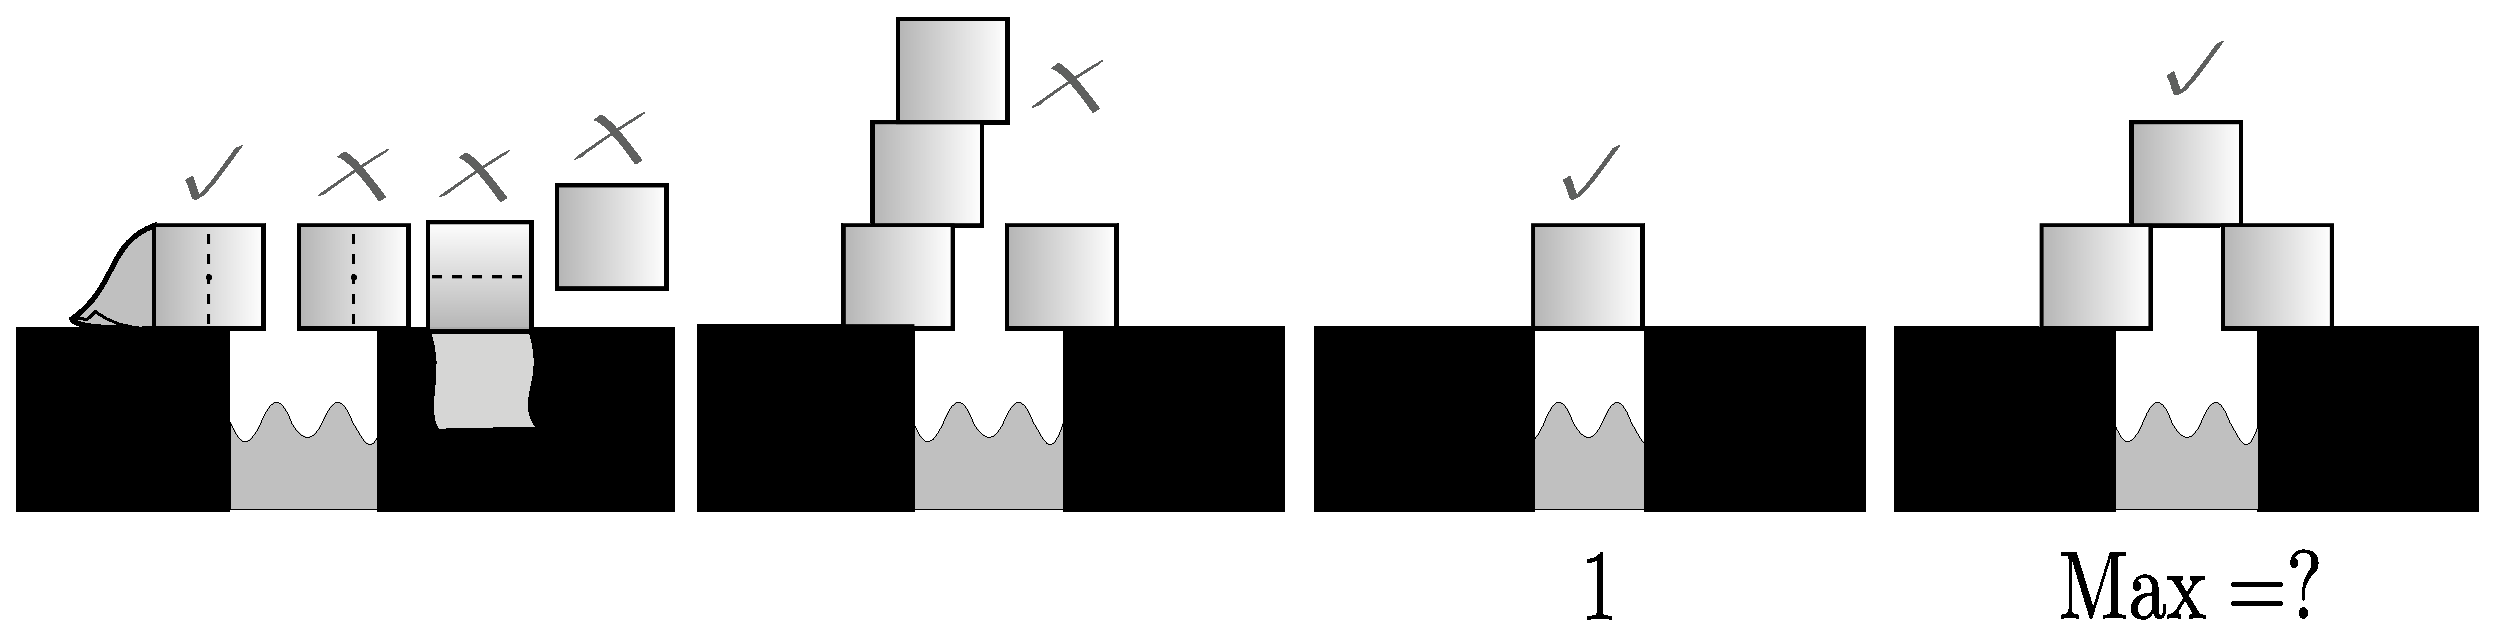
\includegraphics[width = \textwidth]{sources/mosty.eps}

\emph{Názorná ukážka: čo môžete a nemôžete robiť.}

\subsubsection{Podmienky}
\begin{itemize}
    \item Toaleťák musí byť stabilný: pod ťažiskom musí byť iný toaleťák alebo breh, alebo ho musí zhora niečo vhodne pritláčať.
    \item Toaleťáky nesmieme otáčať a~ani sa nesmú len tak vznášať.
    \item Útvar na druhom obrázku nie je most, pretože nie je súvislý.
    \item Na treťom obrázku je optimum pre $N = 1$: dokážeme premostiť rieku ľubovoľnej šírky menšej ako 1.
    \item Na štvrtom obrázku je naozaj most. Aké je jeho rozpätie, to už nechávame zistiť vás :-)
\end{itemize}